\section*{Introduction into Nonlinear Optimization}

\subsection*{Unconstrained Optimization}

\textbf{Problem definition}
Given a set $X\subset R^n$ and a function $f: X \rightarrow R$, determine a $x^* \in X$ with the properties $f(x^*) \leq f(x)$ $\forall x \in X$ for a global minimum and $\forall x$ near $x^*$ for a local minimum, resp.

Necessary and sufficient optimality conditions for a local min.: $\nabla f (x^*) = 0 \Leftrightarrow \norm{\nabla f(x^*)} = 0$, $\nabla^2 f(x*3)$ is positive definite.

\textbf{Rate iterative methods}
Asymptotic rate of convergence: $\lim_{k\to\infty} (\sfrac{\norm{x^{k+1} - x^*}}{\norm{x^k - x^*}^p}) = \epsilon$, where p is the asymptotic order and $\epsilon$ the asymptotic error.
Convergence tests: $\norm{x^{k+1}-x^k}<\epsilon$ and/or $\norm{\nabla f(x^{k+1})}<\epsilon$ for sufficiently large $k$ and small $\epsilon$.

\textbf{Steepest Descent}
Linear convergence. $x^{k+1} = x^{k} + d^k \min_{t \in R}(f(x^k + t d^k))$ with $d^k = -\nabla f(x^k)$.

\textbf{Conjugate Gradient (CG, PCG) methods}
No matrix-matrix mult, only vectors. Solve large systems of eqs. Works only for symmetric positive definite matrices.
$d^{k+1} = -\nabla f(x^{k+1}) + \beta^k d^k$. Search direction better than steepest descent, as there, the angle between search directions can be very small (close Zic-Zac). 
$\beta^k$ either: Plak Ribière: $\beta^k= \sfrac{\nabla f (x^k)^T (\nabla f(x^k) - \nabla f(x^{k-1}))}{\norm{\nabla f (x^{k-1})}^2}$ or Fletcher Reeves: $\beta^k= \sfrac{\norm{\nabla f(x^k)}^2}{\norm{\nabla f (x^{k-1})}^2}$.
Preconditioning (PCG): Cholesky. %\texttt{pcg, ichol, mchol}.

\textbf{Newton Method}
Quadratic convergence. 
Avoids the inversion of the Hessian-matrix by quadratic approximation of the function $f$. The linear system of equations $\nabla^2 f(x^k) d^{k} = -\nabla f(x^k) \Leftrightarrow d^k = - (\nabla^2 f(x^{k}))^{-1} \nabla f(x^k)$ (Newton-equation) is solved instead, to get $x^{k+1}=x^k + d^k$.
No guarantee that a solution exists at the current iteration point. Newton search direction is not necessary a descent direction.
Ensure local convergence by step size strategy and choosing the steepest descent as the search direction at the current iteration $\rightarrow$ descent search direction.

\textbf{Quasi-Newton Method}
Super-linear convergence. No linear system of equations are solved.
Approximate Hessian-Matrix $B^k$. 
Updating formula: Broyden, Fletcher, Goldfarb and Shanno (BFGS) and DFP.
Condition on update: \textit{secant equation}: $B^{k+1} (x^{ki+1}-x^{k}) =B^{k+1} s^{k}=y^{k}= \nabla f^{k+1}-\nabla f^{k}$. 
Displacement $s^k$ and change of gradients $y^k$ must satisfy \textit{curvature condition}, $(s^k)^Ty^k>0$ for symmetric positive definite matrix $B^{k+1}$ map $s^k$ into $y^k$.
Additional requirement for uniqueness: $\min_B(\norm{B-B^k}),$ with $B = B^T, Bs^k=y^k$. 
Different norms $\leftrightarrow$ different Quasi-Newton methods.
BFGS-Method: $B^{k+1} = B^{k} - \frac{B^k s^k (s^k)^T B^k}{(s^k)^T B^k s^k} + \frac{y^k (y^k)^T}{(y^k)^T s^k}$. % not subject of exam

\textbf{Gauss-Newton Method}
Also Q-N. 
Approximation of Newton Method for least squares problem: $\min_{x \in R^n}(f(x))= \frac{1}{2} \norm{F(x)}^2, F: R^n \rightarrow R^m, m \gg n$. 
Convergence rate highly dependent on approximation of Hessian and order of non-linearity of $f$. 
Searching direction by $\nabla f (x) = \nabla F(x)^T F(x)$ $\Rightarrow$ $d_{GN}^k = - (\nabla F(x^k)^T \nabla F(x^k))^{-1} (\nabla F(x^k)^T F(x^k))$

\textbf{Levenberg-Marquardt Method}
Also Q-N. 
Gauss-Newton fails for singular $\nabla F(x^k)^T \nabla F(x^k)$. LM fixes this with trust region radius $\Delta^k$: $\min_{x \in R^n}(f(x))= \frac{1}{2} \norm{F(x^k) + \nabla F(x^k) d^k}^2, \norm{x^k} \leq \Delta^k$. 
If this condition is not fulfilled, it is not equivalent anymore to the Gauss-Newton method, as of the introduction of parameter $\lambda > 0$: $ (\nabla F(x^k)^T \nabla F(x^k) + \lambda \mathbb{1}) d_{LM}^k = - \nabla F(x^k)^T F(x^k)$.

\subsection*{Constrained Optimisation}
Transform constrained problem to a sequence of unconstrained problems. 
Optimality condition not simply performing the first and the second derivative of the objective function anymore.

\textbf{Set of active constraints}: $A(x) = I_{eq} \cup \left\{ i \in I_{in} \mid c_i = 0 \right\}$ 
\textbf{Linear independence constrained qualification LICQ}: The set of active constrained gradients at the solution $\{ \nabla c_i (x^*), i \in A(x^*) \}$ is linearly independent.
\textbf{Feasible directions}: those vectors from the current point that locally satisfy the constraints.
\textbf{Lagrange formulation} of the optimization problem (with $\lambda_i$: Lagrange multiplier): $L(x,\lambda) = f(x) - \sum_{i\in A(x)}\lambda_i c_i (x)$.
\textbf{Critical cone}: $\kappa(x^*, \lambda^*) = \{d \in F(x^*) \mid \nabla c_i (x^*) ^T d = 0, \forall i \in A(x^*) \text{ with } \lambda_i^* > 0$.

\textbf{First order conditions} (for constrained problems): \textit{KKT-conditions}: $\nabla_x L(x^*, \lambda^*) = 0, c_i(x^*) = 0 \forall i \in I_{eq}, c_i (x^*) \geq 0 \forall i \in I_{in}, \lambda_i^* \geq 0 \forall i \in I_{in}, \lambda_o^* c_i (x^*) = 0 \forall i \in I_{eq} \cup I_{in}$. Gradient is $\nabla_x L (x, \lambda) = \nabla_x f(x) - \sum_{i\in A(x)} \lambda_i \nabla_x c_i (x)$

\textbf{Second order conditions} (for constrained problems): KKT-conditions as well as:
For weak local minimum: critical cone: $d^T \nabla_{xx}^2 L(x^* \lambda^*)d \geq 0 \forall d \in \kappa(x^*, \lambda^*)$.  
For strong local minimum: $d^T \nabla_{xx}^2 L(x^* \lambda^*)d > 0 \forall d \in \kappa(x^*, \lambda^*)$

\textbf{Penalty method}
Introduce penalty function: $P(x,a) = f(x) + \frac{\alpha}{2} \sum_i^p c_i^2 (x)$. Solve with $\alpha$ increasing.

\textbf{Sequential quadratic programming (SQP) Method}
One of the most effective for solving nonlinear (small and large) problems including highly nonlinear constraints.
Model the problem $\min_{x\in R^n} f(x), c_i (x) = 0 \forall i \in I_{eq}, c_i (x) \geq 0 \forall i \in I_{in}$ by a quadratic programming subproblem $min_{d \in R^n} (\frac{1}{2} d^T \nabla_xx^2 L (x^k, \lambda^k) d + \nabla f (x^k)^T d + f(x^k)), c_i (x^k) + \nabla c_i (x^k)^T d = 0 \forall i \in I_{eq}, c_i (x^k) + \nabla c_i (x^k)^T d \geq 0 \forall i \in I_{in}$ at each iterate and define the search direction $d$ as the solution of the subproblem.
The new constraints are linearizations of the original constraints
Note: $L(x,\lambda) = f(x) - \sum_{i\in A(x)}\lambda_i c_i (x)$
In constrained gradient based optimization problems, quadratic subproblems have often to be solved $\Rightarrow$ fix with:

\subsection*{Gradient-free methods}
\textbf{Genetic-Algorithms}
Simple, can find global minimum, require lots of function evaluations (but those only). A new generation of individuals is produced using crossover, mutation, ..., operations.

\subsection*{Multiobjective Optimization}
Tradeoff surface (Pareto front): $S$ is a set of values of pair ($f_1$, $f_2$) when x respects the constraints, $P$ is the tradeoff surface.
\textbf{Pareto optimal}: A design variable $x^* \in S$ and the corresponding $f(x^*)$ are pareto optimal if there does not exist another design variable $x\in S$ such that $f_i (x) \leq f_i (x^*) \forall i = 1 ... k$ and $f_j (x) < f_j (x^*)$ for at least one objective function $f_j$.

\begin{figure}
    \centering
    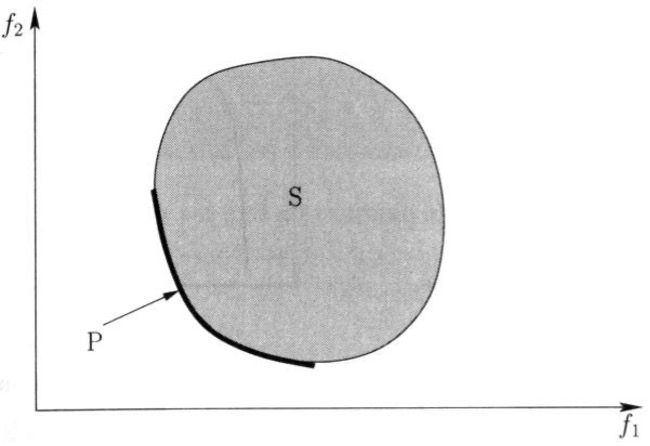
\includegraphics{img/pareto.jpg}
    \caption{Pareto front and set}
    \label{fig:pareto}
\end{figure}

\subsubsection*{Solution methods}
\textbf{Scalar methods}: 
\textit{Weighted sum of objective functions} (only for convex sets $S$): transform problem into monoobjective as $f_{eq}(x) = \sum_{i=1}^k w_i \cdot f_i(x)$ with weights $w_i \geq 0, \sum_{i=1}^k w_i = 1$. 
\textit{Goal attainment method} 
Minimize $\lambda$ with $f_i (x) - w_i \cdot \lambda \leq F_i$ under the constraints. 
$F$ is an initial vector of ideal objective function values and $w$ the search direction/weights. 
The feasible set $S$ is not required to be convex.

% \textbf{Active-Set-Strategy} % not part of exam
